\documentclass[11pt,spanish,a4paper]{article}
% Versión 1er cuat 2014 Víctor Bettachini < bettachini@df.uba.ar >

\usepackage{babel}
\addto\shorthandsspanish{\spanishdeactivate{~<>}}
\usepackage[utf8]{inputenc}
\usepackage{float}
\usepackage{units}
\usepackage{siunitx}
\usepackage{amsmath}
\usepackage{amstext}
\usepackage{amssymb}
\usepackage{graphicx}
\graphicspath{ {./graphs/} {../}}

\voffset-3.5cm
\hoffset-3cm
\setlength{\textwidth}{17.5cm}
\setlength{\textheight}{27cm}

\usepackage{lastpage}
\usepackage{fancyhdr}
\pagestyle{fancyplain}
\fancyhead{}
\fancyfoot{}
\fancyfoot[C]{ {\tiny Actualizado al \today} }
\fancyfoot[RO, LE]{Pág. \thepage/\pageref{LastPage}}
\renewcommand{\headrulewidth}{0pt}
\renewcommand{\footrulewidth}{0pt}


\begin{document}
\begin{center}
	\textsc{\large Física 2 (Físicos)} - Prof. Hernán Grecco\\
	\textsc{\large Primer Cuatrimestre - 2014}\\
	\textsc{\large Guía 6:}	Paquetes de ondas
\end{center}

\begin{enumerate}
\item
\begin{enumerate}
	\item Determine cuáles de las siguientes expresiones matemáticas satisfacen la ecuación de ondas clásica:
	\begin{enumerate}
		\item \(\psi(z,t)= A \mathrm{e}^{-\lambda (a x- b t)^2}\) , \(\lambda \in \mathbb{N} \)
		\item \(\psi(z,t)= A (z+ v t ) \)
		\item \(\psi(z,t)= A \sin{\left( a z+ b t \right) } \)
		\item \(\psi(z,t)= A \sin{\left( a x^2+ b t^2 \right) } \)
	\end{enumerate}
	\item Demueste que cualquier función de la forma \(f(z \pm v t ) \) es solución de la ecuación de ondas clásica.
\end{enumerate}



\item 
	\begin{enumerate}
		\item Demuestre que la suma de dos ondas armónicas de igual frecuencia \( \omega \) que se propagan en la dirección \(+z\), \(A_1 \cos{\left( \omega t - k z + \phi_1 \right) } \) y \( A_2 \cos{\left( \omega t - k z + \phi_2 \right) } \), es una del mismo tipo que puede escribirse como \( A \cos{\left( \omega t - k z + \phi \right) } \).
		Encuentre cómo están relacionados la amplitud \(A\) y fase \(\phi\) de esta última con \(A_1\), \(A_2\), \(\phi_1\) y \(\phi_2\).
		Resuélvalo también en notación compleja y compare ambos resultados.
	\item Ahora calcule la superposición de dos ondas armónicas que se propagan en la dirección \(+z\) de distinta frecuencia, \(A_1 \cos{\left( \omega_1 t - k_1 z + \phi_1 \right) } \) y \(A_2 \cos{\left( \omega_2 t - k_2 z + \phi_2 \right) } \).
		Sepárelas en una portadora a frecuencia promedio multiplicada por la envolvente.
		Verifique en que medida si las frecuencias son iguales o las amplitudes lo son recupera resultados anteriores.
		\item Encuentre el módulo al cuadrado de la envolvente y muestre que evoluciona en el tiempo o en el espacio siguiendo una elipse en el plano complejo.
		¿Cuáles son los valores máximos y mínimos?.
		\item ¿Cómo se propaga la energía de esa superposición?
	\end{enumerate}
		


\item Se superponen una onda de frecuencia \(\omega_0\) de amplitud \(A\) con otras dos de frecuencias corridas en \(\pm \Delta \omega \) de amplitud iguales \(B\).
	\begin{enumerate}
		\item Calcule la envolvente de esta superposición en el origen.
		\item Calcule la envolvente de la onda propagada suponiendo que \( \Delta \omega \ll \omega_o \).
			Discuta que pasa si no vale esta aproximación.
	\end{enumerate}



\item Calcule la velocidad de fase y de grupo para la ecuación de Klein-Gordon.


\item Se encuentra a partir de un modelo\footnote{ver libro \emph{Ondas} de Crawford, cap. 7}  que las ondas superficiales en un líquido satisfacen la siguiente relación de dispersión:
	\[
		\omega^2 = \left( gk + \frac{T}{\rho} k^3 \right) \left[ \frac{ 1- \mathrm{e}^{- 2 k h} }{1+ \mathrm{e}^{- 2 k h} } \right] , \notag
	\]
	donde \(g\) es la aceleración de la gravedad, \(T\) es la tensión superficial (aproximadamente \SI{72d-5}{N/cm} para el agua), \(\rho\) es la densidad del líquido y \(h\) es la profundidad.
	\begin{enumerate}
		\item Encuentre la relación de dispersión en el límite de aguas muy profundas \((h \gg  \lambda) \) y en el opuesto de aguas poco profundas.
		Discuta en que rango de frecuencias y profundidades vale cada aproximación.
		\item Encuentre las velocidades de fase y de grupo en ambos límites.
		\item Se realiza un experimento de propagación de ondas en que se golpea periódicamente la superficie del agua.
			Discuta que se observa en cada caso.
	\end{enumerate}
		
	
\item Calcule y grafique el módulo y la fase de \(C_n\) (coeficientes del desarrollo en serie de Fourier) de la función periódica:
	\begin{center}
		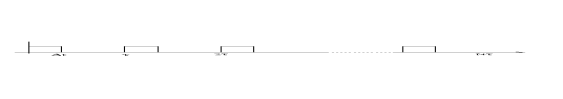
\includegraphics[width=0.75\linewidth]{g06e06}
	\end{center}
	Para:
	\begin{enumerate}
		\item \( \tau= T_1\) y \(\Delta t= \tau_1 \).
		\item \( \tau= 10 T_1\) y \(\Delta t= \tau_1 \).
		\item \( \tau= 100 T_1\) y \(\Delta t= \tau_1 \).
	\end{enumerate}
	Indique una estimación del ancho del espectro de frecuencias para cada caso.



\item Repita lo pedido en el problema anterior para:
	\begin{center}
			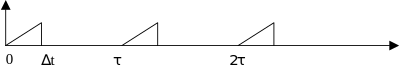
\includegraphics[width=0.75\linewidth]{g06e07}
	\end{center}


\item Calcule como cambia \(C_n\) en los problemas anteriores (6 y 7) si se corre la función en
	una cantidad \(t_o\) hacia la derecha.


\item ¿Cómo cambia la función del tiempo si en los casos de los problemas 6 y 7 se agrega una fase lineal con la frecuencia \(\phi(\omega)= \alpha \omega \) a cada componente \(C_n(\omega_n) \)?

	
\item Si se toma la función de los problemas 6 y 7 como moduladoras o envolventes y se las multiplica por una portadora \(\mathrm{e}^{i \omega_o t} \) (fase lineal con el tiempo),
	\begin{enumerate}
		\item ¿Cómo quedan los nuevos coeficientes de la serie de Fourier.
			Hacer un gráfico cualitativo.
		\item Si dicha perturbación se propaga a derecha con una relación de dispersión 
			\(\omega= c k\), hallar \(\psi(t,z)\).
		\item Ídem. b, si \(\omega= a k+ b\).
			¿A qué velocidad se propaga la portadora y a cuál la envolvente?
	\end{enumerate}

\item Hallar la función del tiempo que tiene como coeficientes de Fourier \(C_n= C\) (constante) para \(n=M\) hasta \(M+N (M \gg N)\).
	Dar el valor de la frecuencia portadora.
	Estimar su ancho temporal.
	Repetir los puntos b y c del problema anterior.


\item Demuestre la siguiente igualdad
	\[
		\int_0^\lambda \mathrm{e}^{i n k x} \mathrm{e}^{- i m k x} \mathrm{d}x = \lambda \delta_{n,m} , 
	\]
	donde n y m son enteros distintos de cero, \(k= \frac{2\pi}{\lambda}\) y \(\delta_{n,m}\) es la delta de Kronecker.


\item Grafique por medio de una computadora la moduladora resultante de superponer 11 ondas de igual amplitud equiespaciadas, si la portadora se toma como la frecuencia más baja, la más alta o la media.
	Discuta la relevancia de las diferencias y como dependen del ancho de banda relativo (relación entre \(\Delta \omega\) y \(\bar{\omega}\)).


\end{enumerate}
\end{document}
